\section{Integral Curves}
Fix $M$ a smooth manifold. 

If $V \in \frak{X}(M)$, then an \textit{integral curve} of $V$ is a smooth curve $\ga:I \to M$ with $\ga'(t) = V_{\ga(t)}$ for all $t \in I$.

Locally, in a chart $(U,\phe)$, we have $\ga^i = x^i \circ \ga$ and $V = V^i \pdv{}{x^i}$, and 
$$\ga'(t) = \dot{\ga}^i(t)\pdv{}{x^i}\bigg|_{\ga(t)}. $$
Then $\ga'(t) = V_{\ga(t)}$ gives a system of ODE
\begin{align*}
&\dot{\ga}^1(t) = V^1(\ga^1(t), \cdots, \ga^n(t)), \\
&\quad \vdots \\
&\dot{\ga}^n(t) = V^n(\ga^1(t), \cdots, \ga^n(t)).
\end{align*}
The fundamental fact about such systems is the existence, uniqueness, and smoothness theorem, from \textbf{Theorem D.1}. of Lee's book. 
\begin{proposition}\label{9.2}
    Let $V \in \frak{X}(M)$, for any $p \in M$ there exists $\eps > 0$ and a smooth curve $\ga:(-\eps,\eps) \to M$ that is an integral curve of $V$ with $\ga(0) = p$.
\end{proposition}
\begin{proof}
    Apply the existence statement to the coordinate representation of $V$. 
\end{proof}
\begin{example}
    Let $(x,y)$ be standard coordinates on $\R^2$, and let $V = \pdv*{}{x}$ be the first coordinate vector field. Then the integral curves of $V$ are precisely the straight lines parallel to the $x$-axis. 
\end{example}
\begin{example}
    Let $\displaystyle{W=x\pdv{}{y} - y\pdv{}{x}}$ on $\R^2$. Let $\ga:\R \to \R^2, \ga(t) = (x(t),y(t))$ be a smooth curve, 
\end{example}


\section{Flows}
Intuitively, flow is the set of all integral curves, which can be viewed as the set of all solutions of an ODE. To specify a point in an integral curve, we need two parameters: initial point $p$ and traveling time $t$ (here we assume curves are defind on $[0,\infty)$ for convenience). 
\begin{figure}[h]
    \centering
    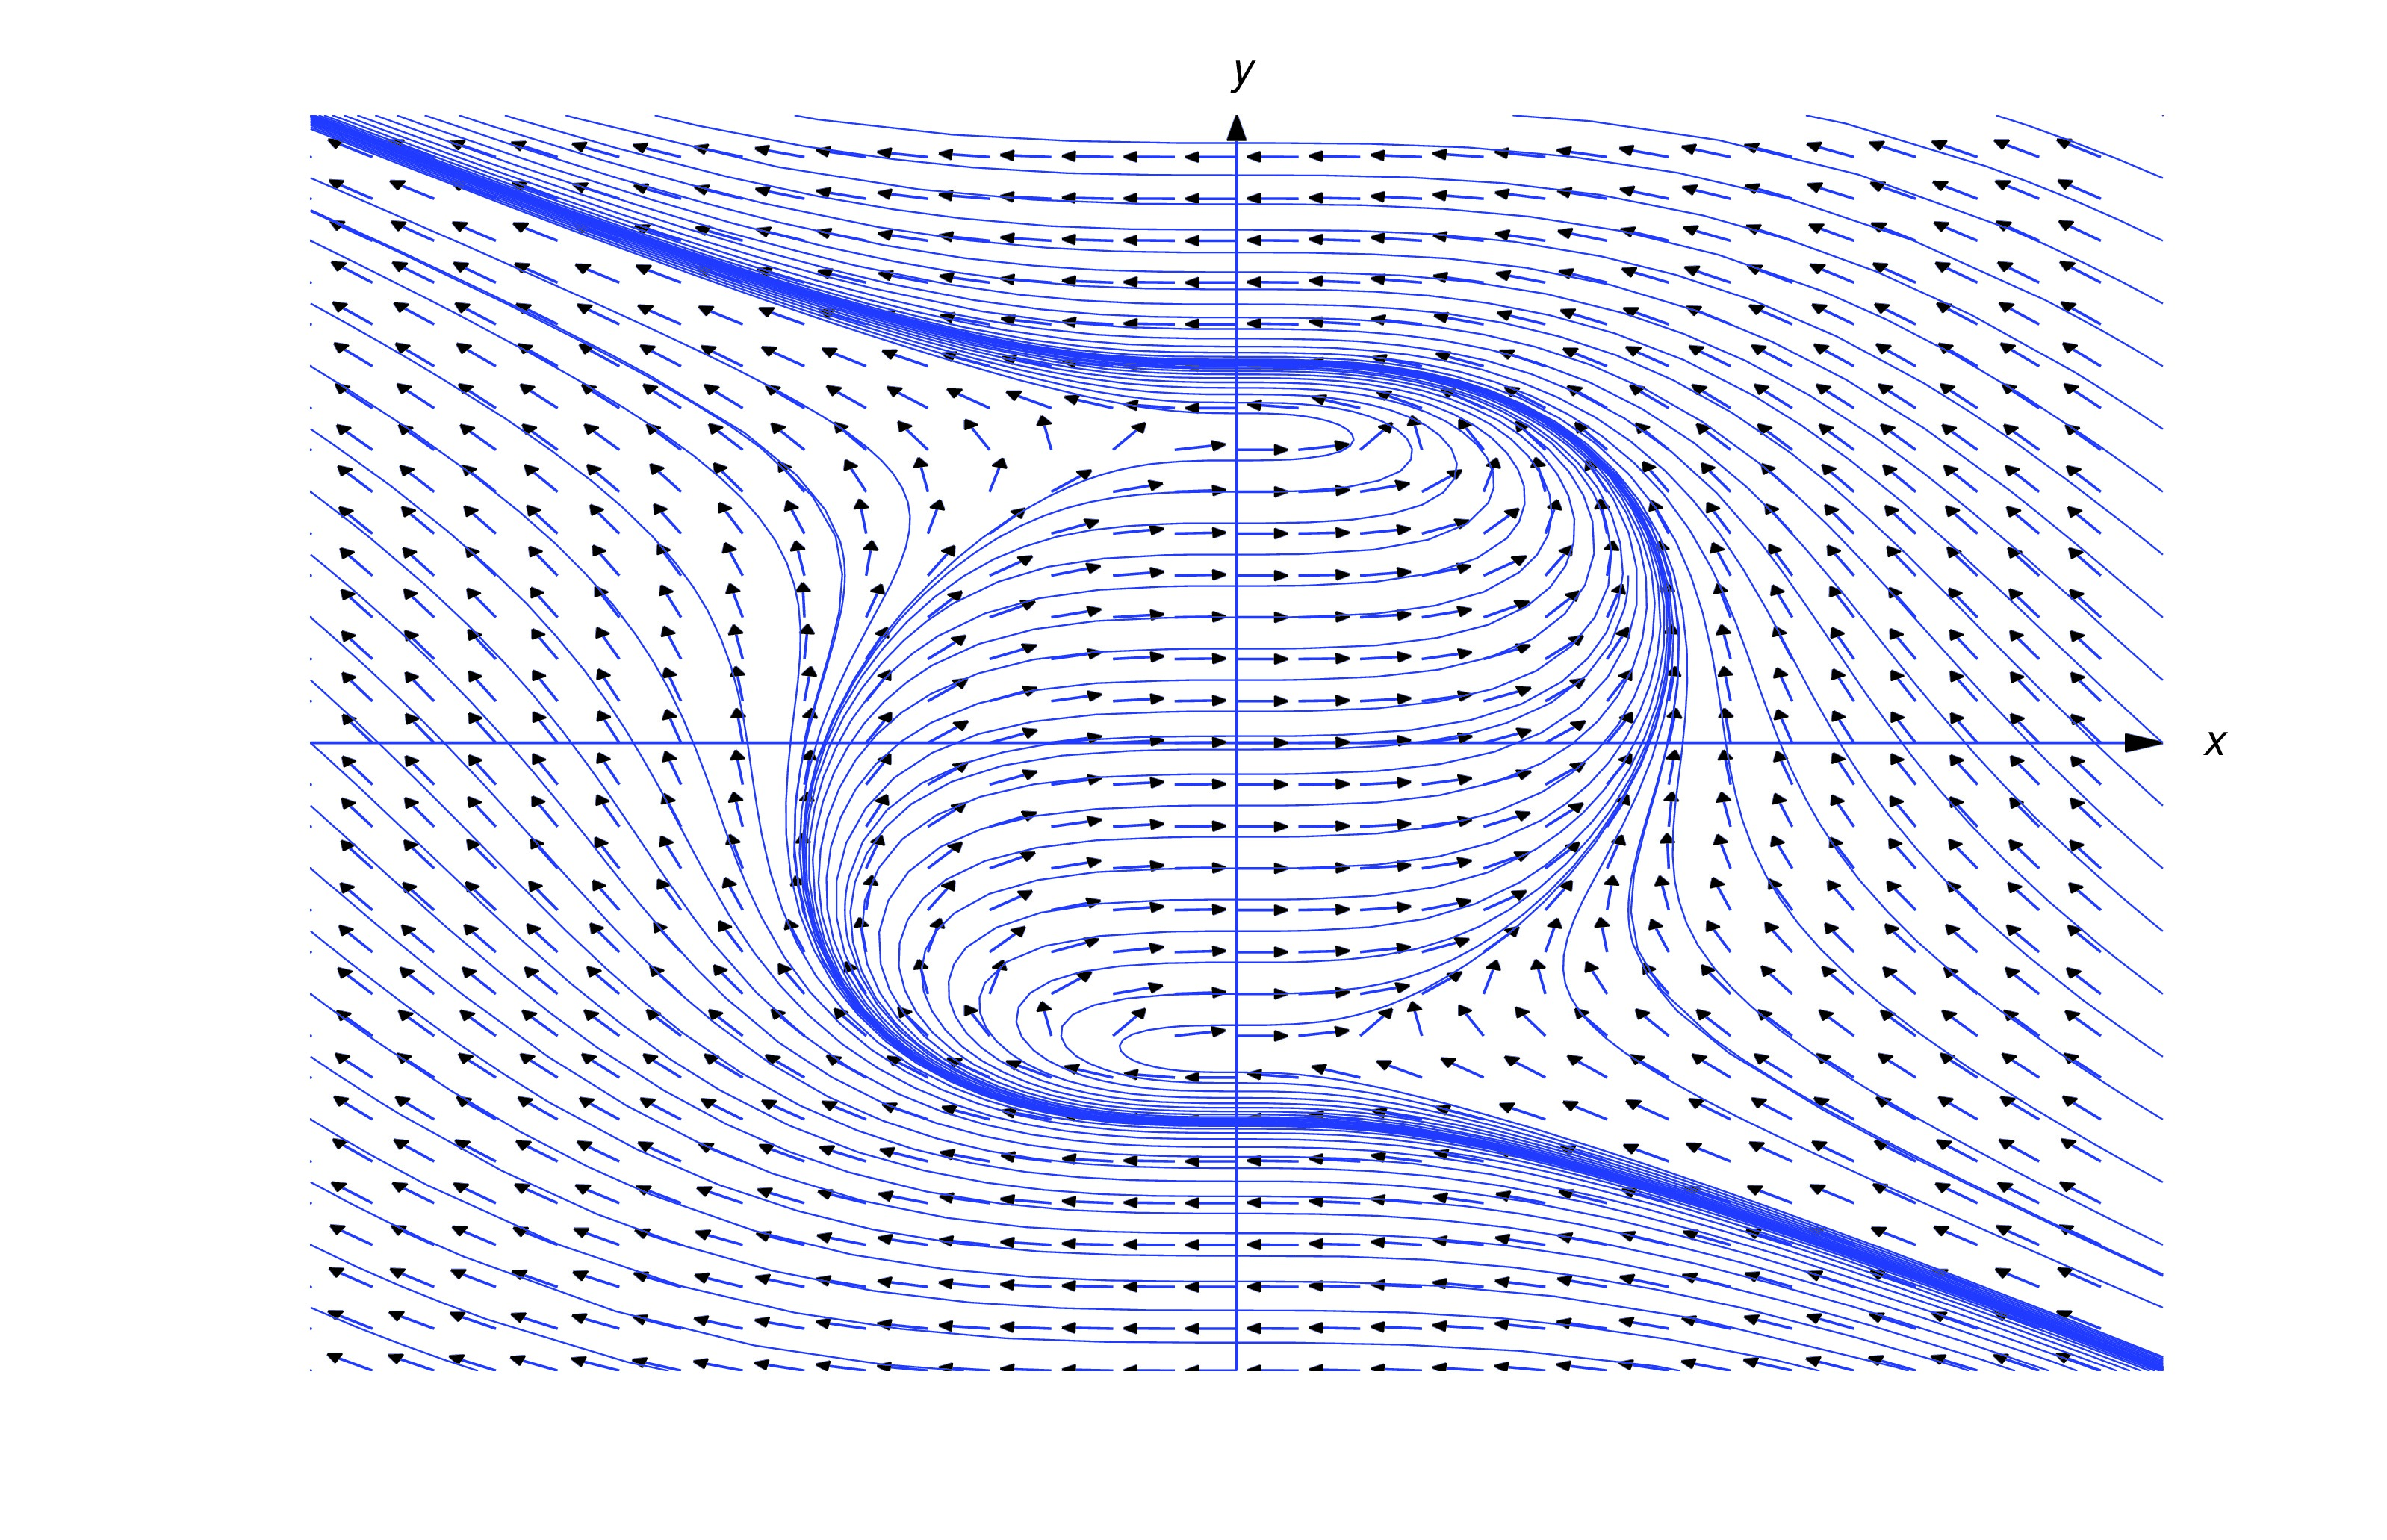
\includegraphics[scale=0.12]{figure/int_curve.jpeg}
    \caption{flow}
\end{figure}
Fix a smooth manifold $M$ and $V \in \frak{X}(M)$. For each $p \in M$, $V$ has a unique integral curve starting at $p$ and defined for all $t \in [0,\infty)$. Now let $p$ runs through all points of $M$, we get a map
\begin{align*}
    \cta: \R \times M &\to M \\
    (t,p) &\mapsto \cta(t,p). 
\end{align*}
Now we can take sections on $\R$ or $M$. 
\begin{itemize}
    \item Fix $p$, we get a map $\cta^{(p)}:\R \to M$ given by $\cta^{(p)}(t) = \cta(t,p)$, which is the point on the curve at time $t$ starting at $p$. This is essentially same as a parametrized curve. 
    \item Fix $t$, we get a map $\cta_t:M \to M$ given by $\cta_t(p) = \cta(t,p)$. This is to see how far can each integral curve travel in time $t$. 
    \begin{figure}[h]
        \centering
        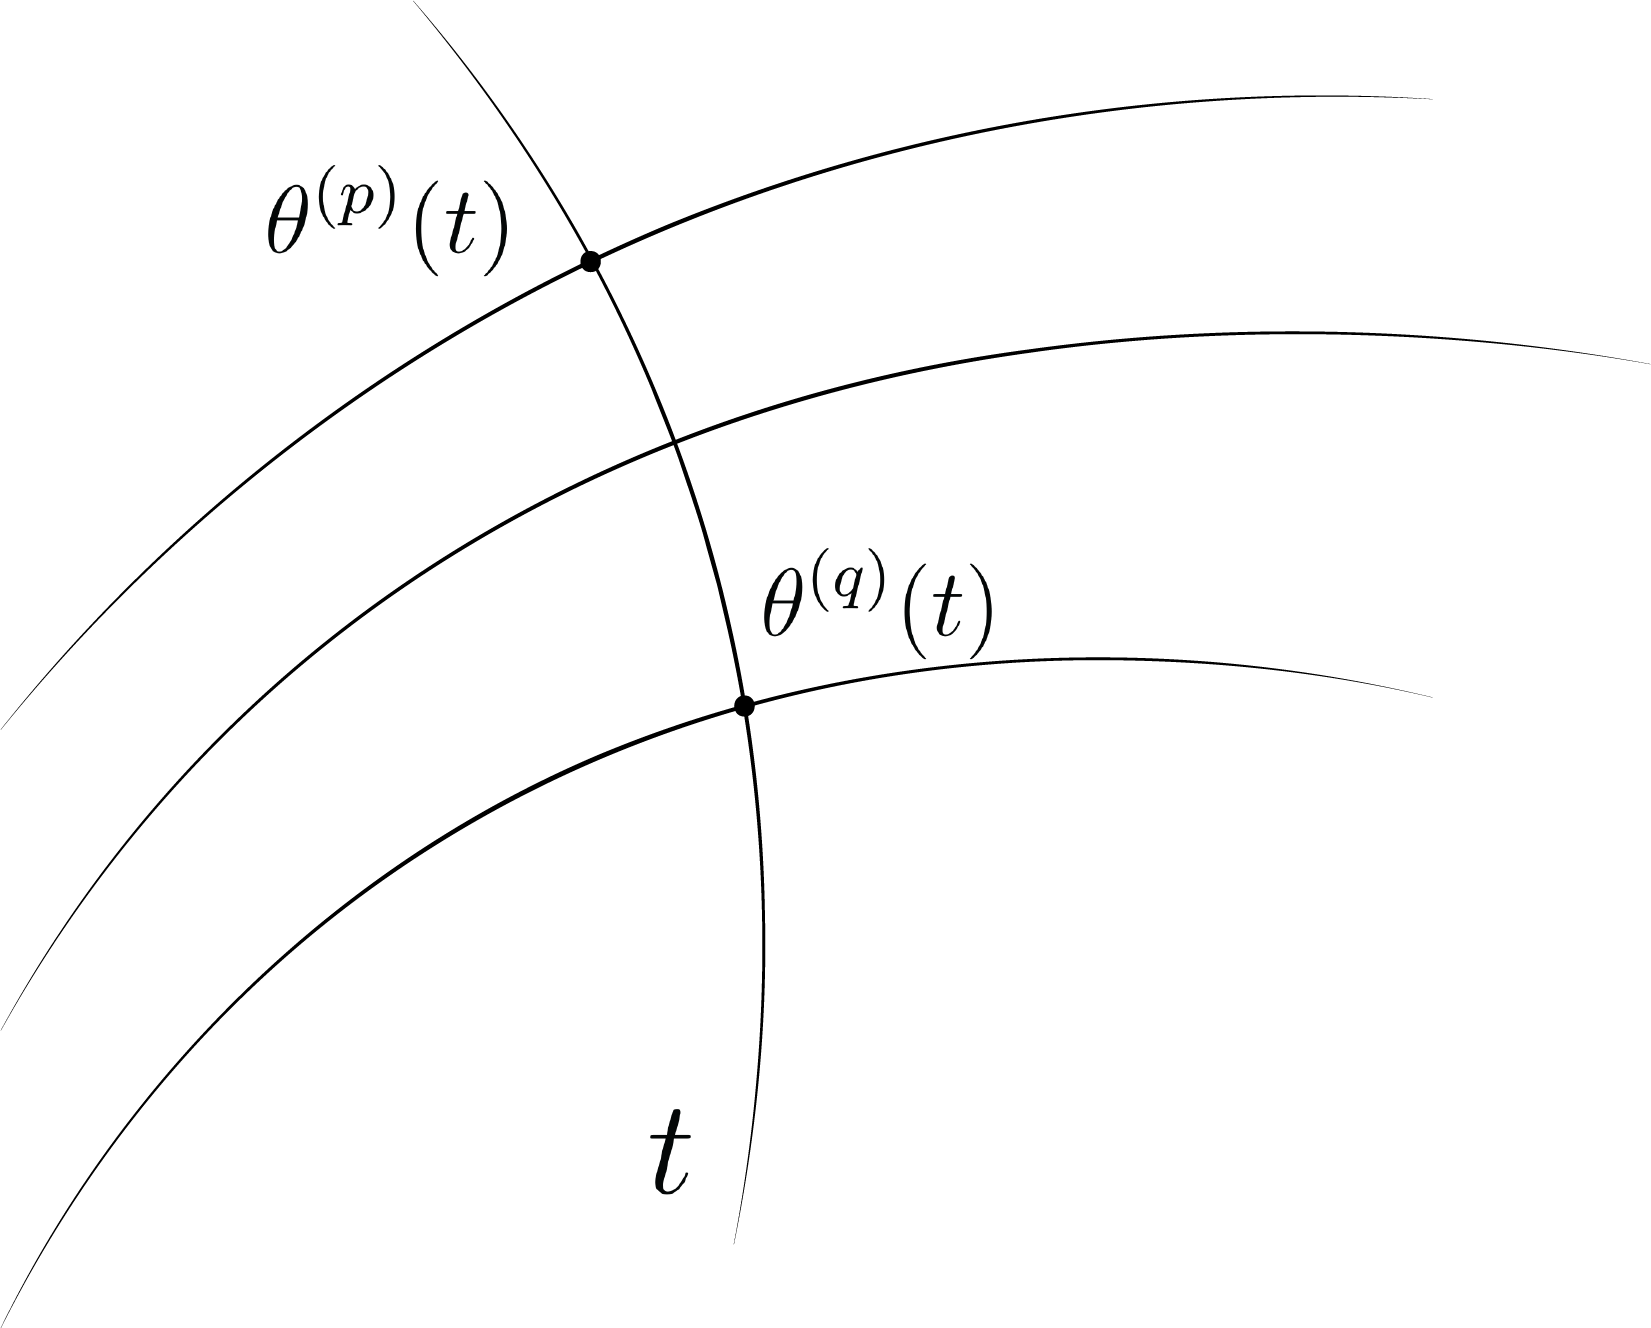
\includegraphics[scale=0.6]{figure/flow.png}
        \caption{Fix $t$, the position $\cta^{(p)}(t)$ and $\cta^{(q)}(t)$}
    \end{figure}
\end{itemize}

Suppose a curve $\cta^{(p)}$ is chosen and let $q$ be another point in this curve: $q = \cta^{(p)}(s)$ for some $s \in (0,\infty)$. By concatenating the time interval $[0, s]$, we can reparametrize $q$ w.r.t. $p$: 
$$\cta^{(q)}(t) = \cta^{(p)}(t+s), \quad t \in [0,\infty). $$
Now $\cta^{(q)}(0) = \cta^{(p)}(s) = q$ is the initial point of $\cta^{(q)}$. In fact, $\cta$ is an action of the group $(\R,+)$ on $M$. To see this, notice that 
\begin{itemize}
    \item $\cta_t \circ \cta_s(p) = \cta_t(\cta_s(p)) = \cta_t(q) = \cta^{(q)}(t) = \cta^{(p)}(t+s) = \cta_{t+s}(p)$.
    \item $\cta_0(p) = \cta^{(p)}(0) = p$. 
\end{itemize}
If we denote the the action by $t \cdot p = \cta^{(p)}(t)$, then 
$0 \cdot p = \cta^{(p)}(0) = p$, and 
$$t \cdot (s \cdot p) = t \cdot (\cta^{(p)}(s)) = t \cdot q = \cta^{(q)}(t) = \cta^{(p)}(t+s) = (t+s) \cdot p. $$
\begin{definition}[global flow]
A \textit{global flow} is a smooth map $\cta:\R \times M \to M$ such that 
\begin{itemize}
    \item $\cta(0,\cdot) = \id_M$,
    \item $\cta(t+s,p) = \cta(t,\cta(s,p))$ for all $s,t \in \R$ and $p \in M$. 
\end{itemize}
\end{definition}
Note that if $\cta_t = \cta(t,\cdot):M \to M$, then the map 
$$t \in (\R,+) \mapsto \cta_t \in \mathrm{Diff}(M)$$ is a homomorphism, since the second property implies that 
$$\cta_{t+s} = \cta_t \circ \cta_s, $$
and $\cta_t^{-1} = \cta_{-t}$ because $\cta_0 = \id_M$.

\begin{center}
    \line(1,0){400} \\[7pt]
    {\Large \textsc{Flow $\to $ Vector Field}} 
    \line(1,0){300} \\[3pt]
\end{center}
It is intuitive that if we take derivative at each point of each integral curve, we will obtain a vector field. 
\begin{definition}
    If $\cta: \R \times M \to M$ is a smooth global flow, for each $p \in M$ we define a tangent vector $V_p \in T_pM$ by 
    $$V_p = {\cta^{(p)}} '(0). $$
    The assignment $p \mapsto V_p$ is a vector field on $M$, which is called the \textit{infinitesimal generator} of $\cta$. 
\end{definition}
\begin{proposition}
    Let $\cta:\R \times M \to M$ be a global flow. Then 
    $$V_p = \dv{}{t}\bigg|_{t=0} \cta(t,p) \in T_pM $$ defines a smooth vector field on $M$. Moreover, each curve $\cta^{(p)}$ is an integral curve of $V$. 
\end{proposition}
\begin{proof}
    Rewrite the expression
    $$V_p = d\cta_{(0,p)}\br{\dv{}{t}\bigg|_{t=0}}, $$
    so $V$ is smooth (in local cooridnates $d\cta_{(0,p)}$ is a matrix whose entries depend smoothly on $p$), hence $V \in \frak{X}(M)$. For the moreover part, fix $p \in M$ and let $\ga(t) = \cta(t,p)$. Then 
    $$\ga'(t) = \dv{}{s}\bigg|_{s=0}\ga(t+s)
    = \dv{}{s}\bigg|_{s=0} \cta(t+s,p) 
    = \dv{}{s}\bigg|_{s=0} \cta(s, \cta(t,p)) 
    = V_{\cta(t,p)} = V_{\ga(t)}. $$
\end{proof}

\begin{center}
    \line(1,0){400} \\[7pt]
    {\Large \textsc{Vector Field $\to $ Flow}} 
    \line(1,0){300} \\[3pt]
\end{center}

Conversely, we would like to be able to say that every smooth vector field is the infinitesimal generator of a smooth global flow, which is not always the case. 
\begin{example}
    Let $M = \R^2 \setminus \{0\}$ and $V$ be the vector field $\pdv*{}{x}$ on $M$. The unique integral curve of $V$ starting at $(-1,0) \in M$ is $\ga(t) = (t-1, 0)$. In this case, $\ga$ cannot be extended continuously past $t=1$. Suppose this were true, let $\widetilde{\ga}$ be any continuous extension of $\ga$ past $t=1$, and notice that $\widetilde{\ga}$ is still a curve in $M = \R^2 \setminus \{0\}$.  
    Then $$\lim_{t \to 1^-}\ga(t) = \widetilde{\ga}(1) \in \R^2 \setminus \{0\}, $$ 
    but if we consider $\ga:M \to \R^2$, then 
    $$ \lim_{t \to 1^-}\ga(t) = \lim_{t \to 1^-} (t-1, 0) = (0,0) \neq \widetilde{\ga}(1), $$ a contradiction. \qed 
\end{example}

It seems that the domain is too large, so we have to restrict integral curves into a \textit{flow domain}.
\begin{definition}[flow domain]
    A \textit{flow domain} $\calD \subset \R \times M$ is an open set such that  for each $p \in M$, the section $\calD^{(p)} := \{t \in \R: (t,p) \in \calD\}$ is an open interval containing $0$. 
    A \textit{(partial) flow} is a smooth map $\cta:\calD \to M$ defined on a flow domain such that $\cta(0,\cdot) = \id_M$ and $\cta(t+s,p) = \cta(t, \cta(s,p))$ whenever both sides are defined. 
\end{definition}

\begin{example}
    Let $\D$ be the open disc in $\R^2$, let $V = \pdv*{}{x}$.
    
    integral curves don't exist for all time.
    Get a flow $\cta:D \to \D$ where $D \neq \R \times \D$.
\end{example}

\begin{definition}
    A \textit{maximal integral curve} is one that cannot be extended to an integral curve on any larger open interval, and a \textit{maximal flow} is a flow that admits no extension to a flow on a larger flow domain (i.e., a flow defined on a maximal flow domain)
\end{definition}

\begin{theorem}[fundamental theorem on Flows]\label{9.12}
    Let $V \in \frak{X}(M)$, there is a unique maximal flow $\cta:\calD \to M$ where $\displaystyle{V_p = \dv{}{t}\bigg|_{t=0} \cta(t,p)}$ for all $p \in M$. Moreover, 
    \begin{enumerate}
    \item for each $p \in M$, 
    $t \in \calD^{(p)} \mapsto \cta(t,p) \in M$ is the unique maximal integral curve starting at $p$.
    \item If $s \in \calD^{(p)}$, then $\calD^{(\cta(s,p))} = \calD^{(p)} \setminus \{s\}$.
    \end{enumerate}
\end{theorem}
\begin{proof}
    Use the existence theorem of an ODE to construct the slice $\calD^{(p)}$, and define a flow domain $\calD$.  
\end{proof}

\begin{definition}
    The flow in \textbf{Theorem \ref{9.12}} is called the \textit{flow generated by} $V$, or just the \textit{flow of} $V$. 
\end{definition}

\section{Complete Vector Fields}
A vector field is \textit{complete} if its flow is a global flow (i.e., defined on $\calD = \R \times M$, so that $\calD^{(p)} = \R$). 
\begin{lemma}[uniform time lemma]\label{9.15} %9.15
    Let $V \in \frak{X}(M)$ and $\cta:\calD \to M$ be the flow of $V$. If there exists $\eps>0$ such that $(-\eps, \eps) \subset \calD^{(p)}$ for all $p \in M$, then $V$ is complete. 
\end{lemma}
\begin{proof}
    Suppose to the contrary that for some $p \in M$, the domain $\calD^{(p)}$ is bounded above. Let $b = \sup \calD^{(p)}$, let $t_0>0$ be such that $b-\eps < t_0 < b$, and let $q = \cta^{p}(t_0)$. The hypothesis implies that $\cta^{(q)}(t)$ is defined at least for $t \in (-\eps, \eps)$. Concatenate $\cta^{(p)}$ and $\cta^{(q)}$ by a curve $\ga:(-\eps, \eps+t_0)$ defined as 
    $$ \ga(t) = \begin{cases}
        \cta^{(p)}(t), & \eps<t<b, \\
        \cta^{(q)}(t-t_0), & t_0-\eps < t < t_0+\eps. \end{cases}$$
    Since by the group law we have 
    $$\cta^{(q)}(t-t_0) = \cta_{t-t_0}(q) = \cta_{t-t_0}\circ \cta_{t_0}(p) = \cta_t(p) = \cta^{(p)}(t), $$
    these two definitions agree where they overlap. By the transition lemma, $\ga$ is an integral curve starting at $p$. Since $t_0+\eps \notin \calD^{(p)}$, this contradicts the maximality of the flow domain.  

    %Fix $p \in M$, then $D^{(p)} = (a,b)$ where $a \in \{-\infty\} \cup (-\infty, 0)$ and $b \in (0,\infty) \cup \{\infty\}$. Suppose for a contradiction that $b \neq \infty$, then $$(-\eps, \eps) \subset D^{(\cta(b-\eps/2, p))} = D^{(p)} \setminus \{b - \eps/2 \} \subset (-\infty, \eps/2), $$
\end{proof}
\begin{corollary} %9.17
    On a compact manifold, every vector field is complete. 
\end{corollary}
\begin{proof}
    See HW 8, Problem 1(a).    
\end{proof}

\begin{lemma}
    Suppose $M$ is a smooth manifold, $V \in \mathfrak{X}(M)$, and let $\theta: \mathcal{D} \rightarrow M$ be the flow of $V$. Then for any compact set $K \subset M$, there exists $\epsilon>0$ such that $(-\epsilon, \epsilon) \times K \subset \mathcal{D}$. 
\end{lemma}
\begin{proof}
    Since $\cta$ is a flow, $\calD$ is a flow domain. Thus for any $p \in M$, $$\calD^{(p)} = \{t \in \R: (t,p) \in \calD\} = (a_p, b_p) \ni 0.$$
    We also have $(a_p, b_p) \times \{p\} \subset \calD$, but $\calD$ is open in $\R \times M$, thus there exists an open set $U_p \ni p$ such that $(a_p, b_p) \times U_p \subset \calD$. For the cover $\{U_p\}_{p \in K}$ we can extract a finite subcover $\bCup{j=1}{n}U_{p_j} \supset K$, and each $U_{p_j}$ corresponds to a 
    $$\calD^{(p_j)} = \{t \in \R: (t,p_j) \in \calD \} = (a_{p_j}, b_{p_j}) \ni 0 $$ and 
    $(a_{p_j}, b_{p_j}) \times U_{p_j} \subset \calD$. Choose $0 < \eps < \min_{1\leq j \leq n} (|a_{p_j}|, |b_{p_j}|)$, we have $(-\eps, \eps) \subset (a_{p_j}, b_{p_j})$ for $j=1, \cdots, n$. Hence 
    $$(-\eps, \eps) \times U_{p_j} \subset \calD \quad \text{ for each } j=1, \cdots, n. $$
    Therefore, 
    $$(-\eps, \eps) \times K \subset (-\eps, \eps) \times \bCup{j=1}{n}U_{p_j} \subset \calD. $$
\end{proof}
\begin{lemma}[escape lemma]\label{9.19}
    If $\ga:J \to M$ is a maximal integral curve of $V$ whose domain $J$ has a finite least upper bound $b$, then for any $t_0 \in J$, $\ga([t_0,b))$ is not contained in any compact subset of $M$. 
\end{lemma}
\begin{proof}
    We may assume that $J = (a,b) \ni 0$. Suppose that there exists $t_0 \in J$ such that $\ga([t_0, b))$ is contained in a compact set $K$ of $M$. Set $p = \ga(a)$, then by the fundamental theorem of flow, there is a maxiaml flow $\cta:\calD \to M$. By uniquenss, $\cta^{(p)}:\calD^{(p)} \to M$ is exactly $\ga$ and $\calD^{(p)} = J$. Let $\{t_n\}_{n=1}^\infty \subset [t_0, b)$ converge to $b$, then $\{\ga(t_n)\}_{n=1}^\infty \subset K$. Then there is a subsequence $\{\ga(t_{n_k})\}_{k=1}^\infty$ with $\ga(t_{n_k})$ converging to some $q \in K$ as $k \to \infty$. By the last lemma, there exists $\eps>0$ such that $(-\eps, \eps) \subset [t_0, b)$ and 
    $(-\eps, \eps) \times K \subset \calD$, so $\cta$ is defined on $(-\eps, \eps) \times K$. Choose $n$ large so that $t_n > b - \eps$, and define $\b:(a, t_n + \eps) \to M$ by 
    $$\b(t) = \begin{cases}
        \ga(t), & a<t<b. \\
        \cta_{t-t_n} \circ \cta_{t_n}(p), & t_n-\eps < t < t_n + \eps.
    \end{cases}$$
    These two definitions agree where they overlap since
    $$\cta_{t-t_n} \circ \cta_{t_n}(p) = \cta_t(p) = \ga(t), $$
    hence $\b$ extends $\ga$ past $b$, a contradiction. 
\end{proof}




\section{Regular Points and Singular Points}
If $V \in \frak{X}(M)$, then $p \in M$ is a \textit{regular point} of $V$ if $V_p \neq 0$. Otherwise, if $V_p=0$, then $p$ is a \textit{singular point} of $V$. 
\begin{theorem}[canonical form near a regular point]\label{9.22}
    If $V \in \frak{X}(M)$, $p \in M$, and $V_p \neq 0$, then there exists a chart $(U,\phe=(x^1,\cdots,x^n))$ centered at $p$ where $V = \pdv*{}{x^i}$ on $U$. 
\end{theorem}
\begin{proof}
    
\end{proof}
\begin{remark}
    No canonical form near singular points: see Lee Figure 9.8.
\end{remark}
\section{Lie Derivatives}
\begin{definition}
    Suppose $V \in \frak{X}(M)$ has flow $\cta$. Then the \textit{Lie derivative} of $W \in \frak{X}(M)$ w.r.t. $V$ is the vector field where 
    $$\calL_V(W) = \dv{}{t}\bigg|_{t=0}d(\cta_{-t})_{\cta_t(p)}(W_{\cta_t(p)})
    = \lim_{t \to 0} \frac{d(\cta_{-t})_{\cta_t(p)}(W_{\cta_t(p)}) - W_p}{t}$$
\end{definition}
\begin{remark}
    $d(\cta_{-t})_{\cta_t(p)}(W_{\cta_t(p)}) \in T_{\cta_{-t}(\cta_t(p))} M$
\end{remark}
\begin{theorem}
    If $V,W \in \frak{X}(M)$, then $\calL_V(W) = [V,W]$. 
\end{theorem}
\begin{proof}
    Fix a chart $(U,\phe)$. In these coordinates 
    $$\cta(t,p) = (\cta^1(t,p), \cdots, \cta^n(t,p)), \quad 
    W = W^j \pdv{}{x^j}. $$
    \begin{align*}
    \calL_V(W) &= \dv{}{t}\bigg|_{t=0} {\pdv{\cta^i}{x^j}}(-t, \cta(t,x)) W^j(\cta(t,x)) \pdv{}{x^i} \\[10pt]
    &= -{\pdv[2]{\cta^i}{t}{x^j}} (-t, \cta(t,x))W^j(\cta(t,x))\pdv{}{x^i} + \pdv[2]{\cta^i}{x^k}{x^j}(-t, \cta(t,x)) {\pdv{\cta^k}{t}}(t,x) W^j(\cta(t,x)) \pdv{}{x^i} \\
    &\quad+ {\pdv{\cta^u}{x^j}} (-t, \cta(t,x)) {\pdv{W^j}{x^k}} (\cta(t,x)) {\pdv{\cta^k}{t}} (t,x) \pdv{}{x^i} \bigg|_{t=0} \\[10pt]
    &= {\pdv[2]{\cta}{t}{x^j}} (0,x) W^j(x) \pdv{}{x^i} + {\pdv[2]{\cta^i}{x^k}{x^j}} (0,x) {\pdv{\cta^k}{t}} (0,x) W^j(x) \pdv{}{x^i} \\
    &\quad+ {\pdv{\cta^i}{x^j}}(0,x) {\pdv{W^j}{x^k}}(x) {\pdv{\cta^k}{t}}(0,x). 
    \end{align*}
    Note 
    $${\pdv{\cta^k}{t}}(0,x) = V^k, \quad {\pdv[2]{\cta^i}{t}{x^j}}(0,x) =  \pdv{}{x^j} \br{{\pdv{\cta^i}{t}}(0,x)} = \pdv{V^i}{x^j}, $$
    and 
    $\cta(0,\cdot) = \id_M$, so 
    \begin{align*}
    &{\pdv{\cta^i}{x^j}}(0,x) = \begin{cases}
    1 & i = j, \\
    0 & i \neq j, \end{cases} \\
    &{\pdv[2]{\cta^i}{x^k}{x^j}} (0,x) = \pdv{}{x^k}\br{ {\pdv{\cta^i}{x^j}}(0,x) } = 0,
    \end{align*}
    then 
    \begin{align*}
    \calL_V(W) = -{\pdv{V^i}{x^j}}W^j\pdv{}{x^i} + 0 + \pdv{W^j}{x^k}V^k\pdv{}{x^j} = [V,W]. 
    \end{align*}
\end{proof}
\begin{corollary}\label{9.39}
    If $V,W,X,Y \in \frak{X}(M)$, then 
    \begin{enumerate}
    \item $\calL_V(W) = -\calL_W(V)$;
    \item $\calL_V([X,Y]) = [\calL_V X,Y] + [X,\calL_V Y]$;
    \item $\calL_{[V,W]}X = \calL_V \calL_W X - \calL_W \calL_V X$.
    \item If $g \in C^\infty(M)$, then 
    $$\calL_V(gW) = (Vg)W + g\calL_V(W).$$
    \item If $F:M \to N$ is a diffeomorphism, 
    $$F_*\calL_V(W) = \calL_{F_* V}(F_* W). $$
    \end{enumerate}
\end{corollary}
\begin{proof}
\begin{enumerate}
    \item $\calL_W(V) = [W,V] = -[V,W]$.
    \item $\calL_V([X,Y]) = [V,[X,Y]]$. Let $f \in C^\infty(M)$, then 
    \begin{align*}
    [V,[X,Y]]f &= V[X,Y]f - [X,Y]Vf \\
    &= V(XYf - YXf) - (XYVf-YXVf) \\
    &= VXYf - VYXf - XYVf + YXVf,
    \end{align*} and 
    \begin{align*}
    [\calL_V X,Y]f &= [[V,X],Y]f \\
    &= [V,X]Yf - Y[V,X]f \\
    &= VXYf - XVYf - YVXf + YXVf, \\
    [X,\calL_V Y]f &= [X,[V,Y]]f \\
    &= X[V,Y]f - [V,Y]Xf \\
    &= XVYf - XYVf - VYXf + YVXf.
    \end{align*}
    \item Similar as (2). 
    \item 
\end{enumerate}

\end{proof}
\section{Commuting Vector Fields}
\begin{definition}
\begin{itemize}
    \item We say that $V,W \in \frak{X}(M)$ are \textit{commute} if $[V,W] = 0$, i.e., $VWf = WVf$ for every smooth function $f$. 
    \item If $\cta:\calD \to M$ is a flow and $W \in \frak{X}(M)$, then $W$ is \textit{invariant} under $\cta$ if \begin{equation}
        d(\cta_t)_p W_p = W_{\cta_t(p)} \quad \text{for all }(t,p) \in \calD
    \end{equation}
    \item Two flows $\cta, \psi$ \textit{commute} if whenever $p \in M$ and $I,J \subset \R$ are open intervals containing $0$ such that one of $\psi_s \circ \cta_t(p)$ or $\cta_t \circ \psi_s(p)$ is defined for all $(s,t) \in I \times J$, then 
    $$\psi_s \circ \cta_t(p) = \cta_t \circ \psi_s(p) $$ for all $(s,t) \in I \times J$ (in particular both defined). 
\end{itemize}
\end{definition}

\begin{theorem} % 9.42 and 9.44
    If $V,W \in \frak{X}(M)$, then TFAE:
    \begin{enumerate}
    \item $V,W$ commute.
    \item $W$ is invariant under the flow of $V$. 
    \item $V$ is invariant under the flow of $W$.
    \item The flows of $V,W$ commute. 
    \end{enumerate}
\end{theorem}
\begin{proof}
    (a) $\iff$ (b). 

    (a) $\iff$ (c): Since $[V,W] = -[W,V]$, this follows from the equivalence of (a) and (b). 

    (b), (c) $\implies$ (d): By symmetry, it suffices to fix $p \in M$ and open intervals $I,J \subset \R$ containing $0$, where $\psi_s \circ \cta_t(p)$ exists for all $(s,t) \in I \times J$, then show that $\psi_s \circ \cta_t(p) = \cta_t \circ \psi_s(p)$ for all $(s,t) \in I \times J$. 
    Fix $s \in I$. Define $\ga:J \to M$ by $\ga(t) = \psi_s \circ \cta_t(p)$. Then $$\ga'(t) = d(\psi_s)_{\cta_t(p)} V_{\cta_t(p)} = V_{\psi_s(\cta_t(p))} = V_{\ga(t)}, $$
    so $\ga$ is an integral curve of $V$. Then $\ga(t) = \cta_t(\psi_s(p))$ for all $t \in J$ since $\ga(0) = \psi_s(p)$. Hence $\cta_t(\psi_s(p)) = \psi_s(\cta_t(p))$ for all $t \in J$. Since $s \in I$ was arbitrary, we are done.

    (d) $\implies$ (b): Fix $p \in M$, then $\psi_s \circ \cta(p) = \cta_t \circ \psi_s(p)$ for $s,t$ small enough. Then $$W_{\cta_t(p)} = \dv{}{s}\bigg|_{s=0}\psi_s(\cta_t(p)) = \dv{}{s}\bigg|_{s=0}\cta_t(\psi_s(p)) = d(\cta_t)_{p}W_p \quad (*) $$
    for $t$ small. To show this for any $t \in D^{(p)}$, use $(*)$ and the fact that 
    $$d(\cta_{t_1+t_2})_p = d(\cta_t)_{\cta_{t_2}(p)}d(\cta_{t_2})_p. $$
\end{proof}

